\renewcommand\drawNodes[2]{
  % #1 (str): namespace
  % #2 (list[list[str]]): list of labels to print in the node of each neuron
  \foreach \neurons [count=\lyrIdx] in #2 {
    \StrCount{\neurons}{,}[\lyrLength] % use xstring package to save each layer size into \lyrLength macro

    \ifthenelse{\equal{#1}{encoder}}{
        \ifnumequal{\lyrIdx}{1}
        {% True case
        \foreach \n [count=\nIdx] in \neurons
            \node[neuron,fill=green,fill opacity=0.2] (#1-\lyrIdx-\nIdx) at (0.7*\lyrIdx, \lyrLength/3.6-0.5*\nIdx) {\n};
        }
        {% False case
        \foreach \n [count=\nIdx] in \neurons
            \node[neuron] (#1-\lyrIdx-\nIdx) at (0.7*\lyrIdx, \lyrLength/3.6-0.5*\nIdx) {\n};
        }
    }{
        \ifnumequal{\lyrIdx}{2}
        {% True case
        \foreach \n [count=\nIdx] in \neurons
            \node[neuron,fill=green,fill opacity=0.2] (#1-\lyrIdx-\nIdx) at (0.7*\lyrIdx, \lyrLength/3.6-0.5*\nIdx) {\n};
        }
        {% False case
        \foreach \n [count=\nIdx] in \neurons
            \node[neuron] (#1-\lyrIdx-\nIdx) at (0.7*\lyrIdx, \lyrLength/3.6-0.5*\nIdx) {\n};
        }
    }
  }
}

\renewcommand\denselyConnectNodes[2]{
  % #1 (str): namespace
  % #2 (list[int]): number of nodes in each layer
  \foreach \n [count=\lyrIdx, remember=\lyrIdx as \previdx, remember=\n as \prevn] in #2 {
    \foreach \y in {1,...,\n} {
      \ifnum \lyrIdx > 1
        \foreach \x in {1,...,\prevn}
          \draw[-] (#1-\previdx-\x) -- (#1-\lyrIdx-\y);
      \fi
    }
  }
}

\begin{tikzpicture}[
    shorten >=1pt, shorten <=1pt,
    neuron/.style={circle, draw, minimum size=2ex, thick},
    legend/.style={font=\large\bfseries},
  ]

  % decoder-a
  \drawNodes{decoder-a}{{{,,}, {,,,}}}
  \denselyConnectNodes{decoder-a}{{3, 4}}

  % decoder-av
  \begin{scope}[yshift=-3.5cm]
    \drawNodes{decoder-av}{{{,,}, {,,,}}}
    \denselyConnectNodes{decoder-av}{{3, 4}}
  \end{scope}
  
%   \node[inner sep=0pt,left of=encoder-1-1,xshift=-0.5cm,yshift=-0.2cm] (input) {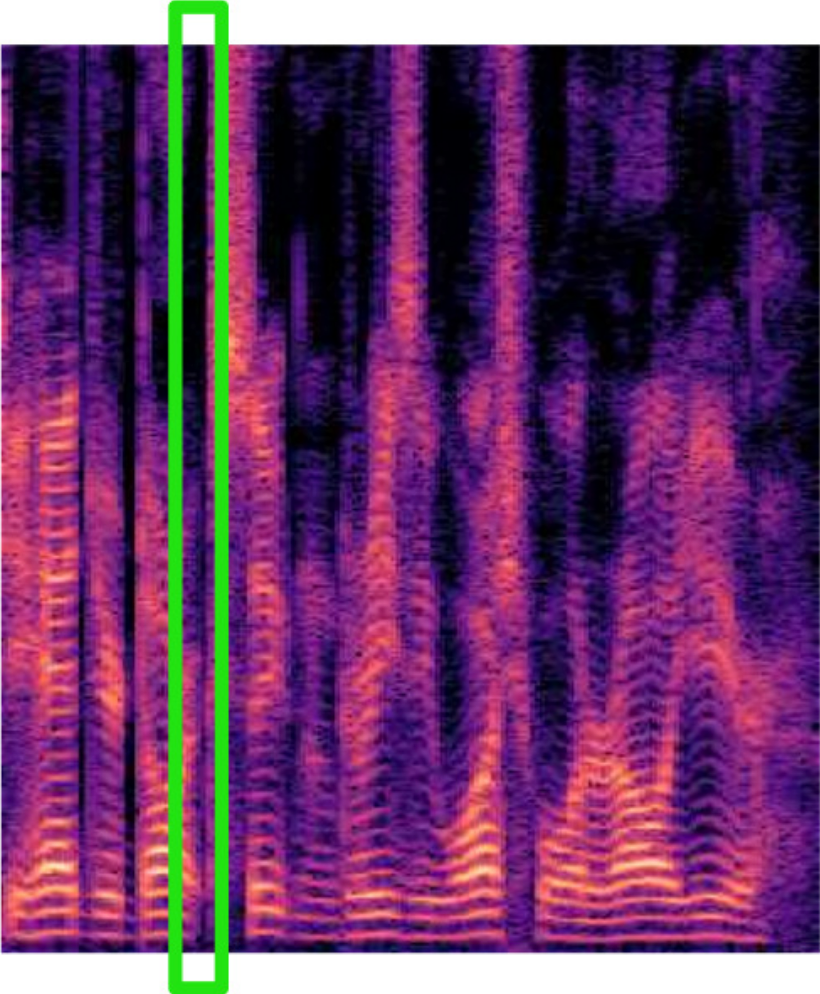
\includegraphics[width=.25\textwidth]{tikz/spectrogram}};
%   \node[inner sep=0pt,left of=encoder-1-1,xshift=-0.5cm,yshift=-2.4cm] (input2) {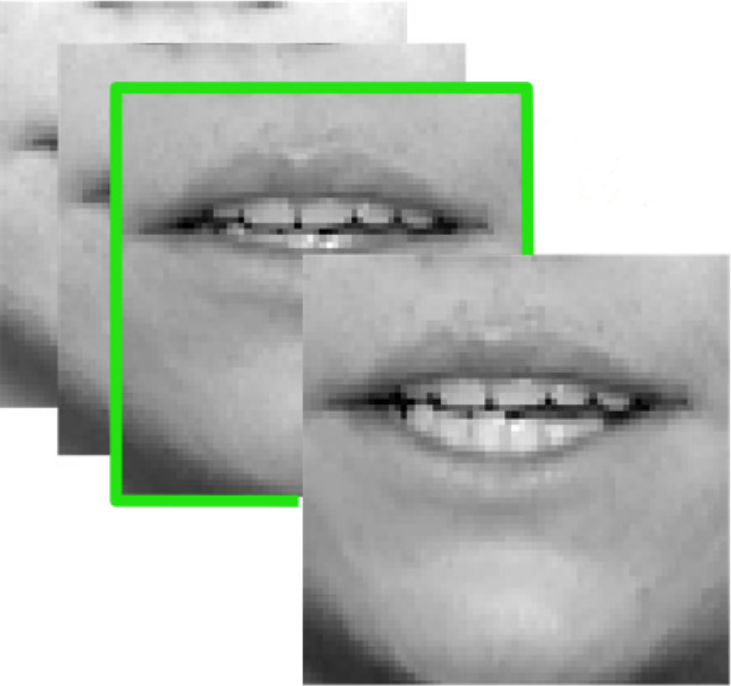
\includegraphics[width=.25\textwidth]{tikz/lips}};
  
  % mu, sigma, sample nodes, conditioning
  \foreach \idx in {1,...,3} {
%       \coordinate[neuron, right=2 of encoder-2-2, xshift=-1.4cm, yshift=0.5*\idx cm-0.15cm, fill=red, fill opacity=0.2] (mu-\idx);
%       \coordinate[neuron, right=2 of encoder-2-2, xshift=-1.4cm, yshift=-0.5*\idx cm+0.15cm, fill=red, fill opacity=0.2] (sigma-\idx);
      \coordinate[neuron, left=of decoder-a-1-\idx, xshift=6mm, fill=red, fill opacity=0.2] (sample-a-\idx);
      \coordinate[neuron, left=of decoder-av-1-1, xshift=6mm, yshift=0.5*\idx cm-0.4cm, fill=red, fill opacity=0.2] (sample-av-\idx);
      \coordinate[neuron, left=of decoder-av-1-1, xshift=6mm,yshift=0.5*\idx cm-2.3cm, fill=green, fill opacity=0.2] (cond-av-\idx);
    }
    
  \node[left=of sample-a-1,xshift=6mm,yshift=-2mm] (post-a) {\textcolor{blue}{Audio-only VAE}};
  \node[below=of post-a,yshift=1cm] {$q^a_{\bs{\phi}}(\bs{\mylz}_n|\bs{\myos}_n,\bs{\myov}_n)$};
  
  \node[left=of sample-av-3,xshift=6mm,yshift=-2mm] (post-av) {\textcolor{magenta}{Audio-Visual VAE}};
  \node[below=of post-av,yshift=1cm] {$q^{av}_{\bs{\phi}}(\bs{\mylz}_n|\bs{\myos}_n,\bs{\myov}_n)$};  
    
  \node[inner sep=0pt,left of=cond-av-1,xshift=-.5cm,yshift=5mm] (cond) {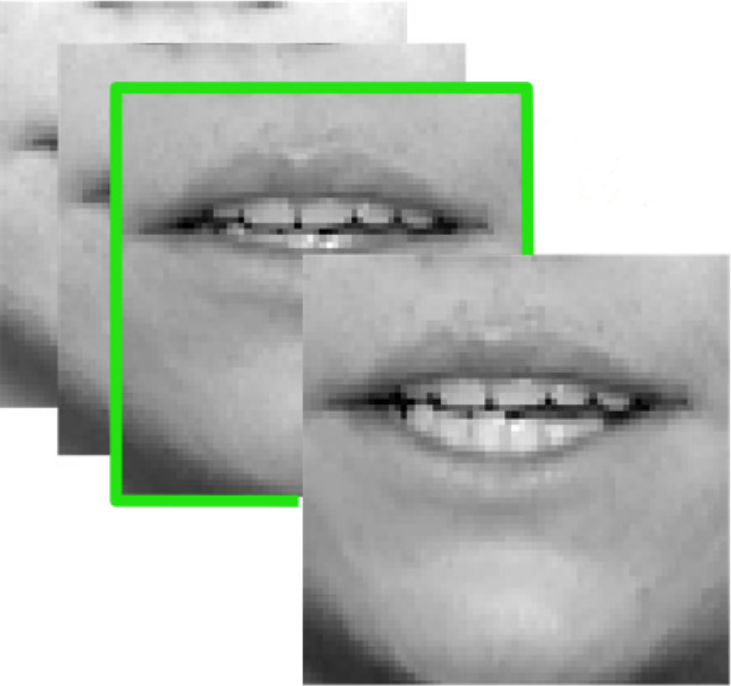
\includegraphics[width=.15\textwidth]{tikz/lips}};

  % mu, sigma, sample boxes
%   \node [label={above:$\bs{\mu}^{av}_{\bs{\mylz}}(\bs{\myos}_n,\bs{\myov}_n)$}, fit=(mu-1) (mu-3), draw] (mu) {};
%   \node [label={below:$\bs{\sigma}^{av}_{\bs{\mylz}}(\bs{\myos}_n,\bs{\myov}_n)$}, fit=(sigma-1) (sigma-3), draw] (sigma) {};
%   \node [fit=(sample-av-1) (sample-av-3), draw] (sample-av) {};
%   \node [fit=(sample-a-1) (sample-a-3), draw] (sample-a) {};

  \node [fit=(decoder-a-2-1) (decoder-a-2-4), draw] (decoder-a-2) {};
  \node [fit=(decoder-av-2-1) (decoder-av-2-4), draw] (decoder-av-2) {};
  \node [fit=(post-av) (sample-av-3) (cond-av-1) (decoder-av-2), draw=magenta, very thick] (vae-av) {};
  \node [fit=(post-a) (decoder-a-2), draw=blue, very thick] (vae-a) {};
  
  \node[circle,draw,below right=of decoder-a-2,yshift=9mm] (alpha) {$\bs{\alpha}_n$};
  \draw[->,blue] (vae-a.east) -- node[above,xshift=8mm] {$p_{\bs{\theta}}(\bs{\myos}_n|\bs{\mylz}^{a}_n)$} ++ (alpha);
  \draw[->,magenta] (vae-av.east) -- node[below,xshift=10mm] {$p_{\bs{\theta}}(\bs{\myos}_n|\bs{\mylz}^{av}_n,\bs{\myov}_n)$} ++ (alpha);
  % mu, sigma, sample connections
%   \draw[dashed] (mu.east) edge (sample.west) (sigma.east) -- (sample.west);
  \foreach \a in {1,2,3}
  \foreach \b in {1,2,3} {
%       \draw[-] (encoder-2-\a) -- (mu-\b);
      \draw[-] (sample-a-\a) -- (decoder-a-1-\b);
      \draw[-] (sample-av-\a) -- (decoder-av-1-\b);
      \draw[-] (cond-av-\a) -- (decoder-av-1-\b);
    }

    \node[inner sep=0pt,right of=alpha,xshift=1.5cm] (output) {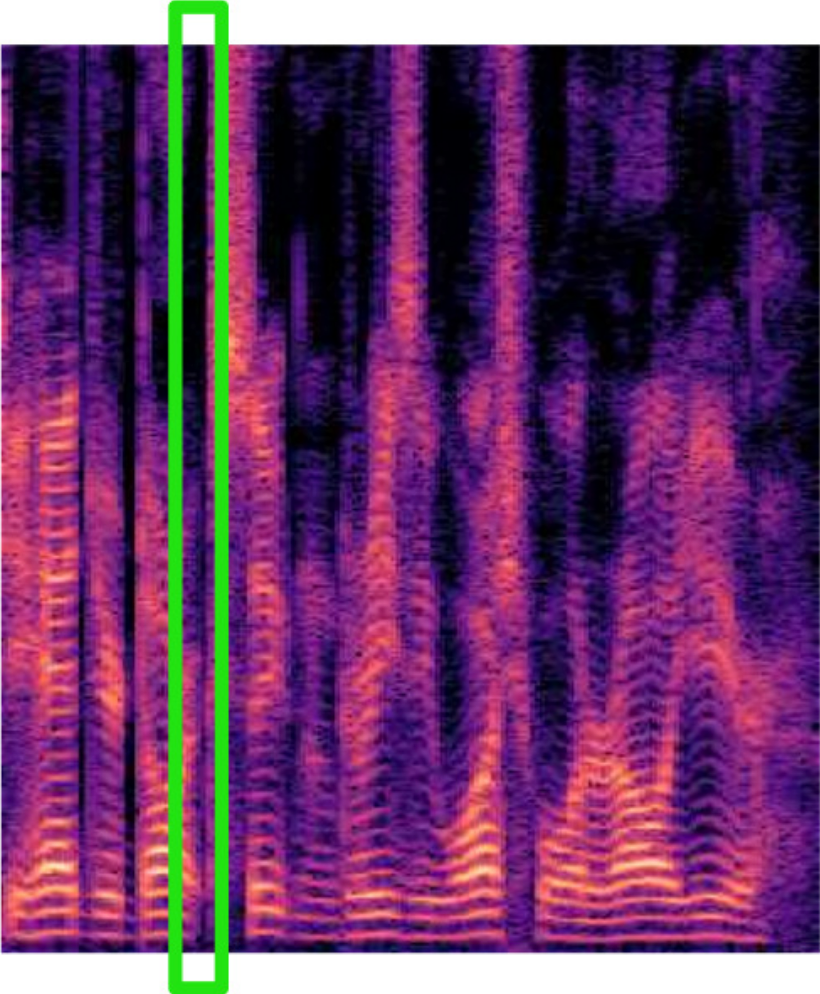
\includegraphics[width=.25\textwidth]{tikz/spectrogram}};
    \draw[->] (alpha) -- (output);
    
  % input + output labels
%   \foreach \idx in {1,...,4} {
%       \node[left=0 of encoder-1-\idx] {$x_\idx$};
%       \node[right=0 of decoder-2-\idx] {$\hat x_\idx$};
%     }
%   \node[above=0.1 of encoder-1-1] {$\bs{\myos}_n$};
%   \node[below=0.1 of encoder-1-6] {$\bs{\myov}_n$};
%   \node[above=0.1 of decoder-a-2-1] {$\hat{\bs{\myos}}_n$};
%   \node[below=0.1 of decoder-av-2-4] {$\hat{\bs{\myos}}_n$};

\end{tikzpicture}
